\documentclass[11pt]{article}
\usepackage[a4paper,margin=0.84in]{geometry}
\usepackage{longtable,booktabs,graphicx,array,amsmath,amssymb,hyperref}
\hypersetup{hidelinks}
\emergencystretch=2.5em
\title{RESTRICTED Technical Evidence and Reproducibility Package\\\large Logistics Cross-Source Reconciliation Manuscript Revision}
\author{Internal authorized review only}
\date{19 November 2026}
\begin{document}
\maketitle
\begin{center}\fbox{\parbox{0.87\linewidth}{\centering\textbf{RESTRICTED --- NOT FOR PUBLICATION OR REPOSITORY UPLOAD}\\Contains actual operational identifiers, code mappings, volumes, and reporting details. Distribute only through an authorized Centre/FedEx-controlled location. Written clearance for the public article is still required.}}\end{center}

\section{Separation of Scope and Evidence}
This package preserves material removed from the proposed public manuscript and adds a fresh independent read-only source-snapshot arithmetic audit. It is \emph{not} an independently verified reconstruction of the historical complete canonicalization, validation, consolidation, or figure-generation workflow. No source-owner field dictionary or shipment-event crosswalk was supplied. The primary source inputs are separately supplied restricted files and are \emph{not} reproduced inside this PDF or ZIP.

\subsection{Status of required external checks}
The exact location of the authoritative source snapshots in Centre/FedEx-controlled storage remains to be confirmed by the data custodian. A second authorized operator must independently rerun \texttt{audit\_compute.py} against the pinned snapshots and record output-hash agreement; any request to certify the historical complete Bronze workflow requires a separately pinned implementation and output chain. The Centre/FedEx disclosure authority must clear the \emph{exact} public PDF, captions, and supplementary materials in writing before submission. Source owners must certify the unit and measurement definition of billed weight and the meaning of the ambiguous origin label; neither is inferred here.

\section{Input Snapshot and Code Manifest}
\subsection{Source snapshot SHA-256 values}
\begin{small}\begin{verbatim}
9f2e1d0f6128475cd02f7b3226e306f8374b673bdf1d8bb468da3668b245ff6b
    input: Weekly 202201-202412(1)(1).xlsx
906bfeba24fcd778e4f17be49542ad75ad7128da0a4335cec0247e674cf2558d
    input: Aug actuals with DOM (1)(1).xlsx
6bd8a4a3fd48f02cba289c5ad1157b9e252f6d21726c59a9ab9c635566bdfb7f
    input: Fedex data version 1 (1)(1).xlsb
\end{verbatim}\end{small}
Input classification: Sources A and B support the direct month-selected count audit. Source C has different coverage and uncertain provenance and is excluded from the main comparison. All snapshots were received as user-provided files; no institutional storage path is certified by receipt here.

\subsection{Exact independent-audit execution}
The new auditable implementation is \texttt{audit\_compute.py}. It reads the original OOXML workbook rows using Python's standard library and applies the explicitly documented date columns, mapping, group-by arithmetic, and source-separated aggregation; it never changes the input workbooks. The executed version uses Python 3.13.5 on Linux. No third-party Python dependencies are required for the numerical audit. Optional figure generation uses \texttt{matplotlib}, separately from the arithmetic.
\begin{verbatim}
python audit_compute.py \
  --weekly "Weekly 202201-202412(1)(1).xlsx" \
  --aug "Aug actuals with DOM (1)(1).xlsx" \
  --xlsb "Fedex data version 1 (1)(1).xlsb" \
  --out restricted_evidence
\end{verbatim}
\noindent The local file paths above are invocation examples, \emph{not} declarations of the approved Centre storage location. The baseline repository commit observed for contextual code review is \texttt{4f18a2fc2d1bd0f568ad9e074da81d5c1f0ed6f9}; this repository contains historical scripts with inconsistent concatenation, zero-fill, and destination-mapping choices. It is not presented as a source of a certified historical publication run.

\noindent Audit script SHA-256:
\begin{small}\begin{verbatim}
ae92d39af3606e8ae1a6de384cebaec4e5c607c46968ad4a82694e52f04f7801  audit_compute.py
\end{verbatim}\end{small}
\subsection{Generated arithmetic output SHA-256 values}
\begin{small}\begin{verbatim}
64d495ab482a8bf9496fccd6bdb40943a21998c2fb1c809aac25435da7727396
    output: count_ledger.csv
a339372ef96ae6f9db1bab3b275afabe8dd42523d4ab5e2ad4fafc259e8eae0d
    output: fixed_population_before_after.csv
761fc2e0030f128fa0bd3640c0528f565b134a13d65bdaa9d6d07777b12ccdc3
    output: reconciliation_destination.csv
c275ee307429238f898ce5265ad6c7a139c9e7cb103e704d1720e6dcf4b66517
    output: reconciliation_service.csv
dd291f3cb92794c0eabd8bce4a5d9dc9e9ac53cd8b10ad0fac5a3ff9d19a5de4
    output: reconciliation_origin.csv
f396e137fbf008a3bbf87a3428684cb01eff00cf18e9f3235142c3216acc9b03
    output: reconciliation_week.csv
4a9a889c091187368dd819b6b491eaed13ea84e73764eda750458782a71f2aee
    output: audit_summary.json
\end{verbatim}\end{small}
The machine-readable \texttt{reproducibility\_manifest.json} contains the exact source and script hashes, output hashes, environment, commands, scope, and named external dependencies.

\section{Restricted Source-Snapshot Audit: Original Tables Relocated from the Manuscript}
\label{sec:verified-reconciliation}
The following audit recalculates values from the supplied, immutable-by-hash raw Excel snapshots, without post-hoc adjustment to manuscript percentages. Source A is the weekly file (\texttt{shp\_dt}) and Source B is the August shipment extract (\texttt{ShipDate}); both are filtered by inclusive dates 2024-08-01 through 2024-08-31. The month selection is based on the records' date columns, not an inclusive whole-fiscal-week rule. In Source A, these are weekly aggregates dated within the month, not individually identifiable source events; consequently the filter cannot establish shipment-level event-set equivalence. No duplicate or validation filter was applied during the raw-record census; this is a baseline snapshot audit, not an assertion about a historically executed production pipeline.

\begin{table}[htbp]\centering\scriptsize
\caption{Direct source-snapshot row conservation before and after mapping.}\label{tab:verified-count}
\begin{tabular}{lr}\toprule
Observation-count ledger & Rows \\
\midrule
Source A: all rows & 168,897 \\
Source A: selected August rows & 7,009 \\
Source B: all rows & 271,802 \\
Source B: selected August rows & 271,802 \\
Source B: mapped-code present & 271,775 \\
Source B: raw code missing & 27 \\
Source B: retained unresolved & 27 \\
Validation exclusions in THIS census & 0 \\
Duplicate removals in THIS census & 0 \\
Source B: post-map retained & 271,802 \\
\bottomrule\end{tabular}\end{table}

\begin{table}[htbp]\centering\scriptsize
\caption{Actual operational destination mappings in Source B; two different raw codes map to Americas.}\label{tab:verified-codemap}
\begin{tabular}{lrr}\toprule
Original code & Canonical lane & Source-B rows \\
\midrule
\texttt{EU} & Europe & 78,783 \\
\texttt{AS} & APAC & 44,142 \\
\texttt{ME} & MEISA & 45,548 \\
\texttt{NA} & Americas & 94,543 \\
\texttt{LA} & Americas & 8,759 \\
Missing code & Unresolved & 27 \\
TOTAL & -- & 271,802 \\
\bottomrule\end{tabular}\end{table}

The verified conservation identity is $271{,}802=271{,}775+27=271{,}802+0+0$. It is a raw-row conservation identity: the 27 missing-code observations carry no usable descriptive lane in the supplied \texttt{Lane} column and are retained as unresolved, not falsely counted as recovered. The pre- and post-map total is unchanged. The former public Figure 1 used different upstream observation populations and is therefore withdrawn. A corrected same-population figure generated from this fixed Source-B selection is contained in Section~\ref{sec:fixedfigure}.

\begin{table}[htbp]\centering\scriptsize
\caption{Recomputed destination-grain package reconciliation (Source A denominator; direct date filtering).}\label{tab:verified-by_lane}
\begin{tabular}{lrrrr}\toprule
Destination & A packages & B packages & $B-A$ & Delta \\
\midrule
\texttt{<MISSING>} & 0 & 34 & 34 & undefined \\
\texttt{APAC} & 83,344 & 83,308 & -36 & -0.043\% \\
\texttt{Americas} & 554,222 & 554,054 & -168 & -0.030\% \\
\texttt{Europe} & 161,156 & 161,422 & 266 & +0.165\% \\
\texttt{MEISA} & 82,147 & 82,617 & 470 & +0.572\% \\
TOTAL & 880,869 & 881,435 & 566 & +0.064\% \\
\bottomrule\end{tabular}\end{table}

\begin{table}[htbp]\centering\scriptsize
\caption{Recomputed service-grain package reconciliation (Source A denominator; direct date filtering).}\label{tab:verified-by_service}
\begin{tabular}{lrrrr}\toprule
Service & A packages & B packages & $B-A$ & Delta \\
\midrule
\texttt{DOM} & 0 & 339 & 339 & undefined \\
\texttt{EF} & 2,630 & 4,793 & 2,163 & +82.243\% \\
\texttt{IE} & 83,724 & 87,382 & 3,658 & +4.369\% \\
\texttt{IP} & 725,131 & 725,125 & -6 & -0.001\% \\
\texttt{PD} & 56,327 & 56,420 & 93 & +0.165\% \\
\texttt{PF} & 7,353 & 7,376 & 23 & +0.313\% \\
\texttt{RL} & 3,503 & 0 & -3,503 & -100.000\% \\
\texttt{RM} & 2,201 & 0 & -2,201 & -100.000\% \\
TOTAL & 880,869 & 881,435 & 566 & +0.064\% \\
\bottomrule\end{tabular}\end{table}

\begin{table}[htbp]\centering\scriptsize
\caption{Recomputed origin-grain package reconciliation (Source A denominator; direct date filtering).}\label{tab:verified-by_ramp}
\begin{tabular}{lrrrr}\toprule
Origin & A packages & B packages & $B-A$ & Delta \\
\midrule
\texttt{BLR} & 115,976 & 115,998 & 22 & +0.019\% \\
\texttt{BOM} & 214,858 & 214,684 & -174 & -0.081\% \\
\texttt{DEL} & 258,946 & 258,963 & 17 & +0.007\% \\
\texttt{DXB} & 291,008 & 291,782 & 774 & +0.266\% \\
\texttt{NA} & 81 & 8 & -73 & -90.123\% \\
TOTAL & 880,869 & 881,435 & 566 & +0.064\% \\
\bottomrule\end{tabular}\end{table}

\begin{table}[htbp]\centering\scriptsize
\caption{Week-number comparison for selected August-dated source rows (weekly reporting dates are not verified shipment-event dates).}\label{tab:verified-week}
\begin{tabular}{lrrr}\toprule
Week number & A packages & B packages & Delta \\
\midrule
31 & 95,079 & 95,371 & +0.307\% \\
32 & 196,388 & 196,207 & -0.092\% \\
33 & 189,400 & 189,523 & +0.065\% \\
34 & 198,314 & 198,557 & +0.123\% \\
35 & 201,688 & 201,777 & +0.044\% \\
\bottomrule\end{tabular}\end{table}

For every category $g$ the exact operation is $100\,(B_g-A_g)/A_g$, where the denominator $A_g$ is the Source-A package sum in that category. Missing categories have $A_g=0$, so the percentage is undefined rather than a finite discrepancy. Both sources have additive package, shipment, and billed-weight measures, but the present tables show package counts, matching the manuscript's key graphical comparisons. The two input workbooks independently yield $880{,}869$ versus $881{,}435$ packages, a net difference of $566$ packages ($+0.06425\%$). For shipments, the corresponding values are $662{,}616$ and $662{,}956$ ($+0.05131\%$). For weight the column names are Source-A \texttt{aPounds} and Source-B \texttt{aLbs}; these are treated as pounds only if their source data dictionaries certify equivalence.

\paragraph{Restricted evidence and reproducibility status.} The supplied input snapshots are fixed by the SHA-256 values in the private accompanying \texttt{verified\_snapshot\_manifest.json}; the independent read-only arithmetic is reproduced by \texttt{audit\_compute.py} and its JSON outputs. This independently recomputes the raw source-snapshot arithmetic; it does not certify historical full-workflow execution, original figure pixels, a locked historical environment, or a second-operator rerun. The additional October--December \texttt{.xlsb} workbook contains different reporting months and is excluded from the August cross-source comparison. Such checks must be logged distinctly from a claim of complete archived historical reproducibility.

\paragraph{Validation-flag overlap status.} The manuscript reports 441 extreme-weight flags, 441 extreme-shipment flags, and 98 zero-activity flags from the separate Bronze validation run. They are marginal counts, not independently verified distinct-record totals. The raw August workbooks are not the identical versioned Bronze QA output, so their content cannot establish the seven Boolean overlap cells. Under the stated positive-threshold/disjoint-zero assumption, a valid distinct-record total is between 539 and 980 inclusive, and must be calculated from original QA row identifiers. As the stated extreme checks use strictly high values and zero-activity requires all measures to be zero, any actual zero-activity row cannot simultaneously satisfy a positive high-value threshold on the same measure: $|W\cap Z|=|S\cap Z|=|W\cap S\cap Z|=0$, assuming the rules are applied to the same records and no threshold is nonpositive. Thus $|W\cup S\cup Z|=980-|W\cap S|$; its exact value is not certified by these three spreadsheets. No invented overlap is reported as observed.


\section{Corrected Figure 1 Evidence from One Population}
\label{sec:fixedfigure}
\IfFileExists{figure1_fixed_population_RESTRICTED.pdf}{\begin{figure}[htbp]\centering
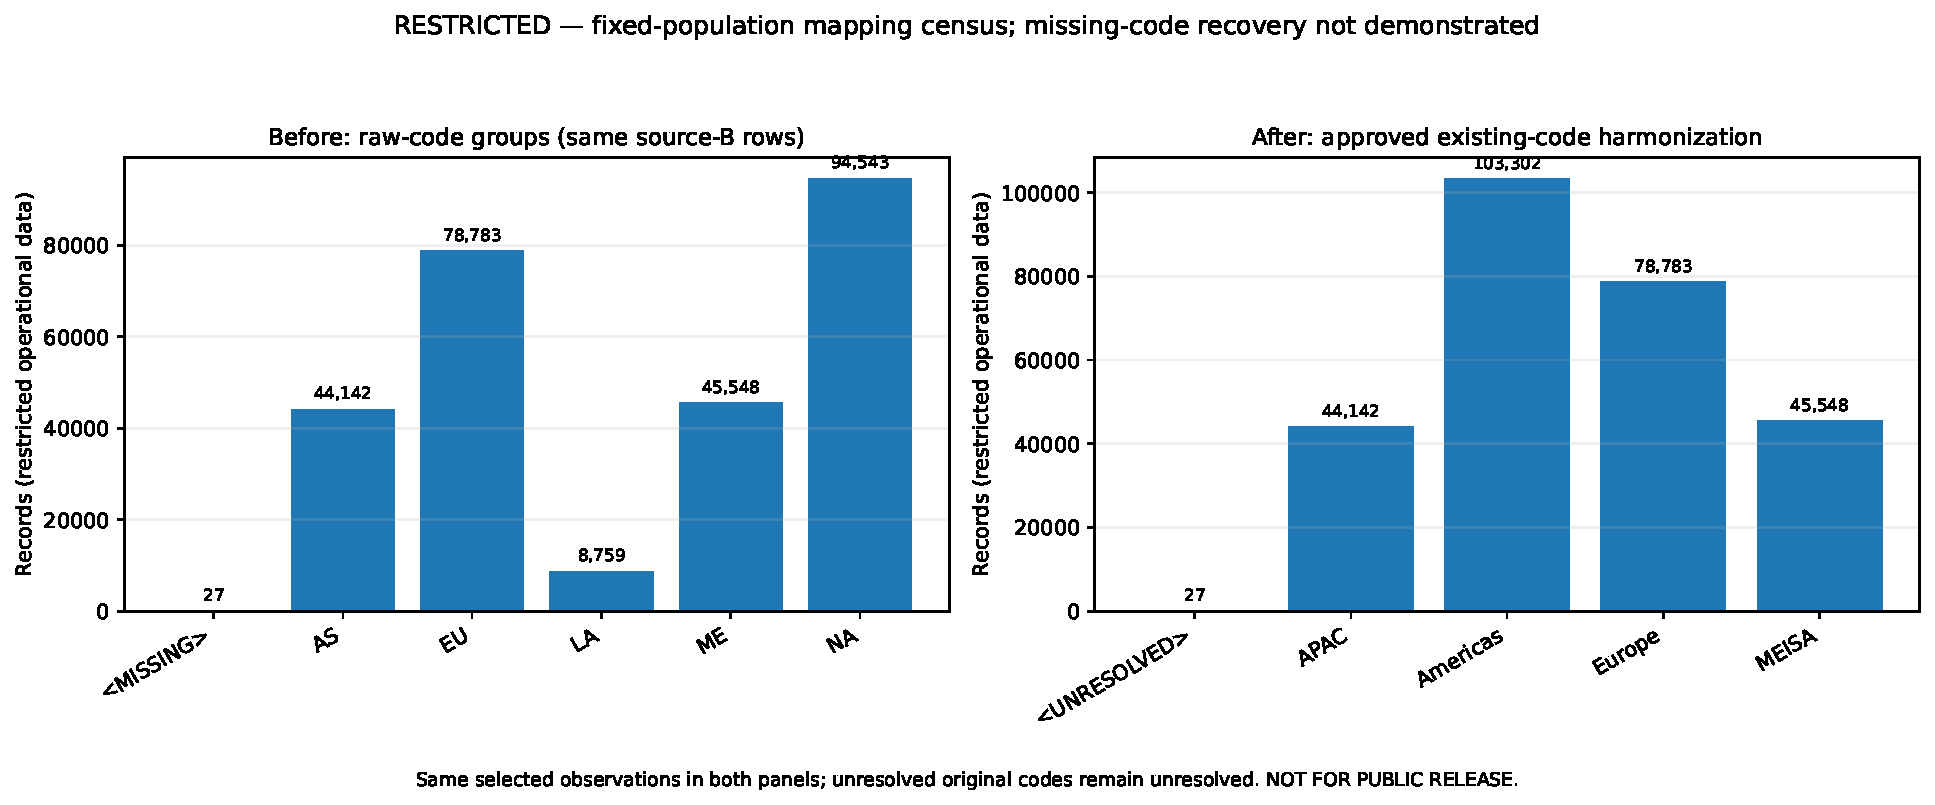
\includegraphics[width=\linewidth]{figure1_fixed_population_RESTRICTED.pdf}
\caption{RESTRICTED. Raw-code and post-map categories are computed on the same Source-B row universe. Existing-code harmonization does not recover the missing codes. All recorded rows remain in the count ledger.}
\end{figure}}{\noindent The accompanying ZIP includes the corrected restricted figure PDF and PNG.}
For this selection, the accounting identity is $271{,}802=271{,}775+0+27+0$: $271{,}775$ existing mapped codes, zero genuinely recovered codes, 27 unresolved missing codes, and zero post-selection exclusions. The previous public panels compared different populations and are removed rather than represented as a valid before/after empirical comparison.

\section{Additional Source-Grain and Coverage Qualifications}
\subsection{Raw seven-field key repetitions}
Among the $7{,}009$ Source-A rows selected by the direct reporting-date filter, the seven-field analytical key has $1{,}979$ distinct combinations and therefore $5{,}030$ surplus occurrences beyond one row per key. This is \emph{not} proof of duplicate shipment events or erroneous repeated rows. It establishes that raw-row uniqueness at the declared seven-field grain cannot be asserted. Aggregation to the exact declared key must precede uniqueness testing; historical Bronze post-aggregation validation cannot be inferred from this source census.

\subsection{Ambiguous additional origin group}
The extra origin group labelled \texttt{NA} appears in both source-specific extracts and is retained in the restricted origin reconciliation. Its business semantics are unconfirmed: it could be a genuine code or a sentinel, and no definition such as ``missing'' or ``North America'' is asserted without a data dictionary. The four named origin-site results are a \emph{subset}, not a complete origin-group summary. The extra group has its own large discrepancy, so a complete-domain maximum is not the four-site maximum. Written owner confirmation of this code's meaning remains pending.

\subsection{Service-category maximum and unmatched categories}
The largest reported absolute finite discrepancy over shared service categories is approximately $82.2\%$, but unmatched Source-A-only service groups have $-100\%$ discrepancies. Therefore $100\%$ is the maximum absolute finite observed service-category discrepancy across all categories whose Source-A denominator is nonzero, and $82.2\%$ can be reported only as a \emph{shared-category} maximum. A Source-B-only category has a zero Source-A denominator, so its signed percentage is undefined rather than zero. This distinction is reflected in the public method but the actual category results are excluded pending disclosure clearance.

\subsection{Source precedence and overlap}
The arithmetic audit separately sums the date-selected Source-A and Source-B records. It does \emph{not} add these sums to create a combined operational total. The control used here is source A as reference and source B as comparison-only in the overlapping calendar window. Historical \texttt{scripts/bronze\_kpi\_weekly\_table.py}, \texttt{scripts/fedex\_adapter.py}, and \texttt{scripts/fedex\_adapter\_2.py} use concatenation and are not evidence of an overlap-free unified output. No assertion of zero duplicates follows from the absence of a historical, immutable, keyed-output rerun.

\subsection{Weight equivalence and temporal scope}
A report-date filter and an event-date filter identify source-specific month-selected populations, not necessarily identical shipments. The audit does not implement a period-allocation crosswalk. Weight-field renaming alone is insufficient evidence of equivalent billed-weight definitions or units. Accordingly, numerical billed-weight reconciliation is removed from the proposed public paper. Required owner confirmations are not replaced by inferred units.

\section{QA Flag Set Overlap and Record-Level Evidence}
The historical Bronze validation marginal counts were $|W|=441$, $|S|=441$, and $|Z|=98$. The raw source files supplied for this audit are not the immutable row-level validation output that produced these flags. Assuming the all-zero definition and strictly positive extreme thresholds were executed on the same observations, $Z$ is disjoint from both high-value sets. Thus $|W\cup S\cup Z|=980-|W\cap S|$, and $0\le|W\cap S|\le441$ implies the possible distinct count range $539\text{--}980$. The intersection and distinct total are unverified. If the positive-threshold/disjoint-set assumption fails, the bound must be recomputed from row-level flag identifiers; no exact unique total is asserted.

\section{Exhibit-Level Confidentiality and Reproducibility Mapping}
The accompanying \texttt{exhibit\_disclosure\_inventory.csv} enumerates every empirical table or figure present in the previous manuscript, its proposed location, whether the result was removed or restricted, the generating artifact where available, and its clearance status. The main report retains no numeric operational empirical exhibits. Public schematic or purely methodological tables require the same final publication-package review but do not contain measured operational quantities.

The accompanying count ledger, fixed-population before/after census, and category-level reconciliation CSV files are direct outputs of the new \texttt{audit\_compute.py} execution. The historical derived-output QA artifacts have not been reconstructed; row-level flag overlap is a named missing dependency. All output hashes appear in the manifest. An authorized reviewer must rerun from approved copies and record hash agreement independently; this package documents a local first run only.

\section{Pending Custodian Confirmation Record}
\begin{enumerate}
\item \textbf{Data custodian / Centre:} provide an authorized storage path, source-snapshot access control, and confirmation that the pinned hashes represent sanctioned inputs.
\item \textbf{Reporting-source owners:} confirm date, fiscal-week and period-allocation rules, shipment-population semantics, weight-unit equivalence, and interpretation of the \texttt{NA} origin value.
\item \textbf{Independent authorized reviewer:} rerun the new audit and any proposed complete canonicalization output and sign the comparison of output hashes. Provide row-level QA identifiers to establish exact flag overlaps.
\item \textbf{SMART Centre/FedEx publication authority:} approve or deny the exact proposed public PDF, captions, references, availability language, and all proposed supplementary artifacts in writing.
\item \textbf{Centre/project lead:} confirm the sanctioned project-title wording preserved in the acknowledgment; no second insertion was made.
\end{enumerate}
\end{document}
